\UseRawInputEncoding
\documentclass[a4paper, 14pt]{extarticle}

% Поля
%--------------------------------------
\usepackage{geometry}
\geometry{a4paper,tmargin=2cm,bmargin=2cm,lmargin=3cm,rmargin=1cm}
%--------------------------------------


%Russian-specific packages
%--------------------------------------
\usepackage[T2A]{fontenc}
\usepackage[utf8]{inputenc} 
\usepackage[english, main=russian]{babel}
%--------------------------------------

\usepackage{textcomp}

% Красная строка
%--------------------------------------
\usepackage{indentfirst}               
%--------------------------------------             


%Graphics
%--------------------------------------
\usepackage{graphicx}
\graphicspath{ {./images/} }
\usepackage{wrapfig}
%--------------------------------------

% Полуторный интервал
%--------------------------------------
\linespread{1.3}                    
%--------------------------------------

%Выравнивание и переносы
%--------------------------------------
% Избавляемся от переполнений
\sloppy
% Запрещаем разрыв страницы после первой строки абзаца
\clubpenalty=10000
% Запрещаем разрыв страницы после последней строки абзаца
\widowpenalty=10000
%--------------------------------------

%Списки
\usepackage{enumitem}

%Подписи
\usepackage{caption} 

%Гиперссылки
\usepackage{hyperref}

\hypersetup {
	unicode=true
}

%Рисунки
%--------------------------------------
\DeclareCaptionLabelSeparator*{emdash}{~--- }
\captionsetup[figure]{labelsep=emdash,font=onehalfspacing,position=bottom}
%--------------------------------------

\usepackage{tempora}
\usepackage{amsmath}
\usepackage{color}
\usepackage{listings}
\lstset{
  belowcaptionskip=1\baselineskip,
  breaklines=true,
  frame=L,
  xleftmargin=\parindent,
  language=Python,
  showstringspaces=false,
  basicstyle=\footnotesize\ttfamily,
  keywordstyle=\bfseries\color{blue},
  commentstyle=\itshape\color{purple},
  identifierstyle=\color{black},
  stringstyle=\color{red},
  extendedchars=\true,
}

%--------------------------------------
%			НАЧАЛО ДОКУМЕНТА
%--------------------------------------

\begin{document}

%--------------------------------------
%			ТИТУЛЬНЫЙ ЛИСТ
%--------------------------------------
\begin{titlepage}
\thispagestyle{empty}
\newpage


%Шапка титульного листа
%--------------------------------------
\vspace*{-60pt}
\hspace{-65pt}
\begin{minipage}{0.3\textwidth}
\hspace*{-20pt}\centering

\includegraphics[width=\textwidth]{emblem}
\end{minipage}
\begin{minipage}{0.67\textwidth}\small \textbf{
\vspace*{-0.7ex}
\hspace*{-6pt}\centerline{Министерство науки и высшего образования Российской Федерации}
\vspace*{-0.7ex}
\centerline{Федеральное государственное бюджетное образовательное учреждение }
\vspace*{-0.7ex}
\centerline{высшего образования}
\vspace*{-0.7ex}
\centerline{<<Московский государственный технический университет}
\vspace*{-0.7ex}
\centerline{имени Н.Э. Баумана}
\vspace*{-0.7ex}
\centerline{(национальный исследовательский университет)>>}
\vspace*{-0.7ex}
\centerline{(МГТУ им. Н.Э. Баумана)}}
\end{minipage}
%--------------------------------------

%Полосы
%--------------------------------------
\vspace{-25pt}
\hspace{-35pt}\rule{\textwidth}{2.3pt}

\vspace*{-20.3pt}
\hspace{-35pt}\rule{\textwidth}{0.4pt}
%--------------------------------------

\vspace{1.5ex}
\hspace{-35pt} \noindent \small ФАКУЛЬТЕТ\hspace{80pt} <<Информатика и системы управления>>

\vspace*{-16pt}
\hspace{47pt}\rule{0.83\textwidth}{0.4pt}

\vspace{0.5ex}
\hspace{-35pt} \noindent \small КАФЕДРА\hspace{50pt} <<Теоретическая информатика и компьютерные технологии>>

\vspace*{-16pt}
\hspace{30pt}\rule{0.866\textwidth}{0.4pt}
  
\vspace{11em}

\begin{center}
\Large {\bf Лабораторная работа № 6} \\ 
\large {\bf<<Вычисление сил тока в электрической цепи методом узловых потенциалов>>} \\ 
\large {\bf по курсу <<Численные методы линейной алгебры>>} \\ 
\end{center}\normalsize

\vspace{8em}


\begin{flushright}
  {Студент группы ИУ9-71Б Лысенко В. В.\hspace*{15pt} \\
  \vspace{2ex}
  Преподаватель Посевин Д. П.\hspace*{15pt}}
\end{flushright}

\bigskip

\vfill
 

\begin{center}
\textsl{Москва 2024}
\end{center}
\end{titlepage}
%--------------------------------------
%		КОНЕЦ ТИТУЛЬНОГО ЛИСТА
%--------------------------------------

\renewcommand{\ttdefault}{pcr}

\setlength{\tabcolsep}{3pt}
\newpage
\setcounter{page}{2}

\section{Цель работы}\label{Sect::task}
\par
\renewcommand{\labelenumii}{\arabic{enumi}.\arabic{enumii}.}
Построить и вычислить СЛАУ, характеризующую электрическую цепь выданного варианта. Найти силы тока в цепи. 

\section{Задачи}\label{Sect::task}
\par
\renewcommand{\labelenumii}{\arabic{enumi}.\arabic{enumii}.}
\begin{enumerate} 
    \item Построить СЛАУ, характеризующую электрическую цепь (20 вариант).
	\begin{center}
		
\includegraphics[scale=0.35]{g1}
	\end{center}
    \item Произвести вычисления письменно.
    \item Сверить полученые результаты с результатами смоделированной электрической цепи (сайт https://falstad.com/circuit/)
    \item Реализовать программу, строящую и вычисляющую СЛАУ для данной электрической цепи.
    \item Сверить результаты, полученные писменно, из программы и из модели.
\end{enumerate}

\pagebreak
\section{Практическая реализация}
\par
Ниже представлен ход вычисленний, проведённых письменно:
\par
\begin{center}

\includegraphics[scale=0.35]{g2}
\par

\includegraphics[scale=0.30]{g3}
\end{center}

\par
Модель электрической цепи:
\begin{center}
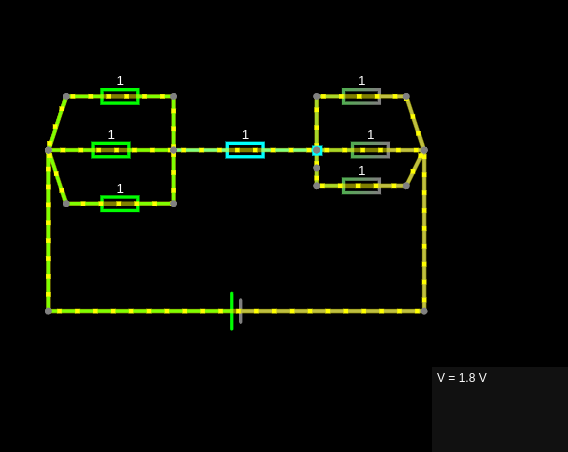
\includegraphics[scale=0.75]{g4}
\end{center}

\par
Код программы:
\begin{lstlisting}
using LinearAlgebra

R121 = 1.0
R122 = 1.0
R123 = 1.0

R231 = 1.0

R341 = 1.0
R342 = 1.0
R343 = 1.0

z = 9.0


A = [0.0 0.0 0.0 1.0;
     1.0 0.0 0.0 -1.0;
     -(1/R121 + 1/R122 + 1/R123) (1/R231 + 1/R121 + 1/R122 + 1/R123) -(1/R231) 0.0;
     0.0 (1/R231) -(1/R231 + 1/R341 + 1/R342 + 1/R343) (1/R341 + 1/R342 + 1/R343)]
A = Float64.(A)

F = [0.0 z 0.0 0.0]
F = Float64.(F)

for i in 1:4
    for j in 1:4
        print(A[i, j], " ")
    end
    println()
end
println()

println(F)
println()

X = A \ F'


println("phi-vector: ")
for j in 1:4
    print(X[j], " ")
end
println()

println()
println("I121 : ", (X[1]-X[2])/R121)
println("I122 : ", (X[1]-X[2])/R122)
println("I123 : ", (X[1]-X[2])/R123)
println()
println("I231 : ", (X[2]-X[3])/R231)
println()
println("I341 : ", (X[3]-X[4])/R341)
println("I342 : ", (X[3]-X[4])/R342)
println("I343 : ", (X[3]-X[4])/R343)
\end{lstlisting}

\section{Результаты}
\par
Результат выполнения программы:
\begin{center}
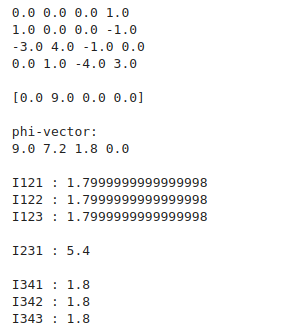
\includegraphics[scale=0.85]{g5}
\end{center}
\par
Зныченя в электрической цепи:
\begin{center}
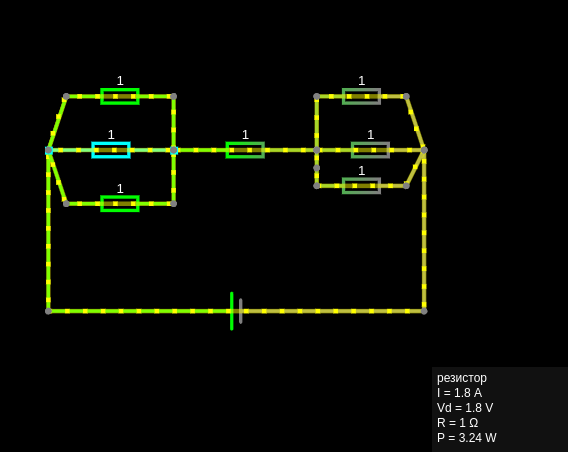
\includegraphics[scale=0.75]{g6}
\end{center}
\par
\begin{center}
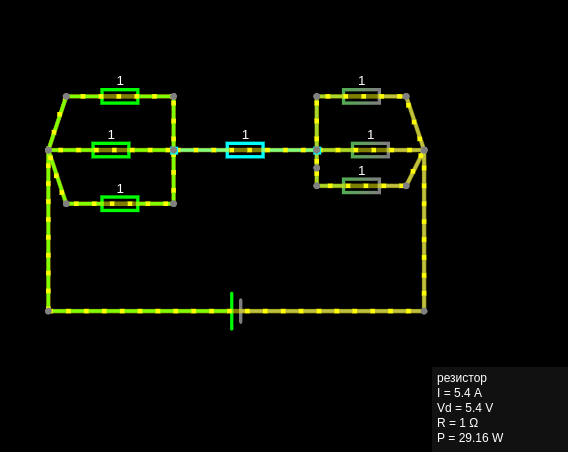
\includegraphics[scale=0.75]{g7}
\end{center}
\par

\section{Выводы}
В ходе выполнения лаборатороной работы была построена и вычислена СЛАУ, а также найдены силы тока в предоставленной в индивидуальном варианте электрической цепи. Был подробно изучен метод узловых потенциалов. Результаты вычислений, полученные письменно и программно успешно сошлись с полученными из модели электрической цепи.
\end{document}
